\documentclass[11pt]{standalone}
\usepackage{amssymb}
\usepackage{amsmath}
\usepackage[no-math]{fontspec}
\usepackage{unicode-math}
\usepackage{libertinus}
\usepackage{pgf,xcolor}
\usepackage{tikz}
\usetikzlibrary{arrows.meta, backgrounds}
\usepackage{pgfplots}
\pgfplotsset{compat=newest}

\definecolor{my_darkgray}{HTML}{484949}
\definecolor{my_lightgray}{HTML}{F3F4F4}
\definecolor{my_darkblue}{HTML}{005A94}
\definecolor{my_lightblue}{HTML}{CCDEE9}
\definecolor{my_yellow}{HTML}{FFEC7F}
\definecolor{my_red}{HTML}{E60000}
\definecolor{my_orange}{HTML}{E87846}

\begin{document}
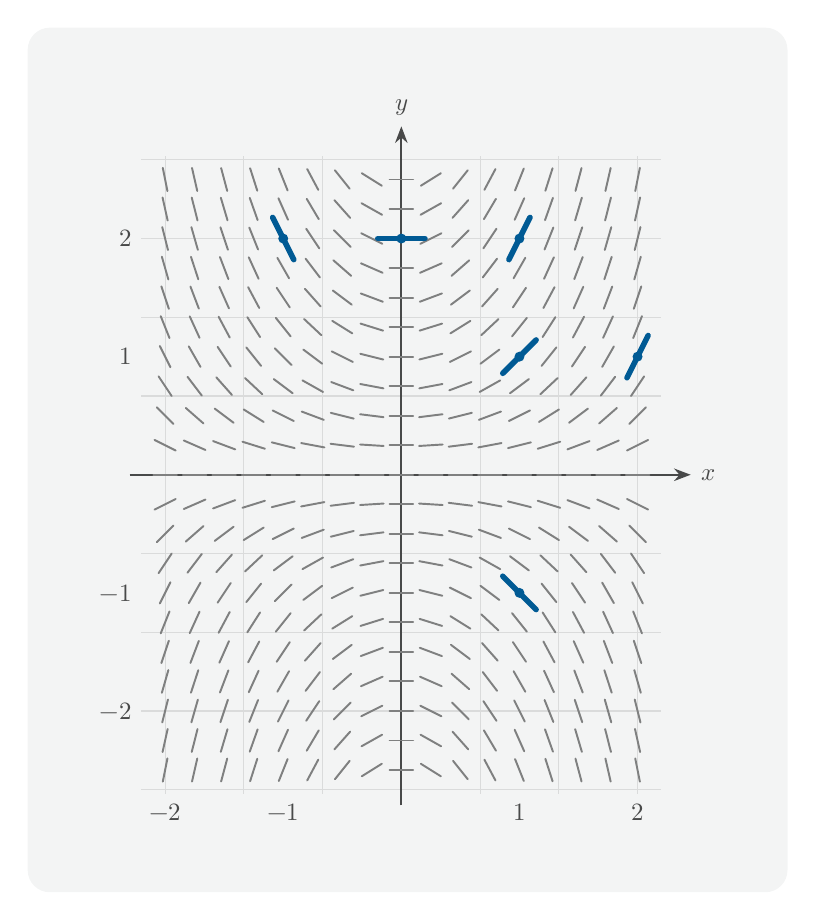
\begin{tikzpicture}[
    show background rectangle,
    background rectangle/.style={fill=my_lightgray, rounded corners=8pt},
    inner frame sep=0.8cm,
    x=1.5cm, y=1.5cm
]
% ---------------------------------------------------------------
%  Richtungsfeld der DGL y' = x y auf [-2, 2] x [-2.5, 2.5],
%  Gitter mit Abstand 0.25, Linienelemente mit gleicher Laenge.
%  Hervorgehoben (dunkelblau) die Punkte der Wertetabelle in 8.3:
%  (0, 2): 0, (1, 1): 1, (1, 2): 2, (2, 1): 2, (-1, 2): -2, (1, -1): -1.
% ---------------------------------------------------------------

\draw[my_darkgray!20, thin] (-2.2, -2.7) grid (2.2, 2.7);

\draw[-{Stealth[length=6pt]}, thick, my_darkgray] (-2.3, 0) -- (2.45, 0)
    node[right, font=\small] {$x$};
\draw[-{Stealth[length=6pt]}, thick, my_darkgray] (0, -2.8) -- (0, 2.95)
    node[above, font=\small] {$y$};
% Beschriftungen am Rand, damit sie das Feld nicht verdecken
\foreach \t in {-2, -1, 1, 2}{
    \node[below, font=\small, my_darkgray] at (\t, -2.7) {$\t$};
    \node[left, font=\small, my_darkgray] at (-2.2, \t) {$\t$};
}

% Linienelemente
\foreach \x in {-2, -1.75, ..., 2.01}{
    \foreach \y in {-2.5, -2.25, ..., 2.51}{
        \pgfmathsetmacro{\m}{\x*\y}
        \pgfmathsetmacro{\dx}{0.1/sqrt(1 + \m*\m)}
        \pgfmathsetmacro{\dy}{\m*\dx}
        \draw[my_darkgray!70, line width=0.7pt, line cap=round]
            (\x - \dx, \y - \dy) -- (\x + \dx, \y + \dy);
    }
}

% Hervorgehobene Linienelemente aus der Wertetabelle
\foreach \x/\y in {0/2, 1/1, 1/2, 2/1, -1/2, 1/-1}{
    \pgfmathsetmacro{\m}{\x*\y}
    \pgfmathsetmacro{\dx}{0.2/sqrt(1 + \m*\m)}
    \pgfmathsetmacro{\dy}{\m*\dx}
    \draw[my_darkblue, line width=2pt, line cap=round]
        (\x - \dx, \y - \dy) -- (\x + \dx, \y + \dy);
    \fill[my_darkblue] (\x, \y) circle[radius=1.8pt];
}

\end{tikzpicture}
\end{document}
